%!TEX root = ../memoire.tex

\chapter{GenDR}\label{chapgendr}

GenDR (Generic Deep Realizer) est un réalisateur profond multilingue \citep{lareau18}. Il a hérité de l'architecture de MARQUIS \cite{WannerMARQUISGENERATIONUSERTAILORED2010} que nous avons présenté à la section \ref{sectionmarquis}. GenDR modélise le langage dans des paramètres similaires à ceux de son prédecesseur. La réalisation linguistique se fait via la transduction de graphes, la théorie Sens-Texte est aussi le cadre utilisé, et les mécanismes permettant la transduction de graphes (dictionnaires et règles de grammaire) fonctionnent essentiellement de la même manière. GenDr a aussi repris la \ac{TST} \citep{melcuk1988},\citep{MelcukSemanticsmeaningtext2012} comme théorie linguistique car c'est une théorie qui a fait ses preuves en matière de \ac{GAT} si on se fie à MARQUIS \citep{WannerMARQUISGENERATIONUSERTAILORED2010}, FORGe \citep{MilledemoFORGePompeu2017}, RealPro \citep{LavoieFastPortableRealizer1997} qui l'utilisent. De plus, \cite{Vicentegeneracionlenguajenatural2015} mentionne ce cadre théorique comme étant une bonne interface pour modéliser le langage dans un article concernant l'état de l'art en \ac{GAT}.

GenDR se démarque par sa capacité à traiter des phénomènes langagiers complexes: les collocations. Il offre une couverture beaucoup plus importante que MARQUIS en ce qui concerne les collocations via un traitement exhaustif des fonctions lexicales. Cette couverture lexicale a été opérée par Lareau et Lambrey \cite{LambreyImplementationcollocationspour2017}, \cite{lambrey15} en travaillant sur un générateur de collocations. Toutefois, il est important de préciser que GenDR réalise en sortie des structures syntaxiques de surface. Le réalisateur se concentre principalement sur l'interface sémantique-syntaxe car c'est là qu'on peut modéliser des phénomènes langagiers profonds. Pour compléter la réalisation jusqu'à du texte, il faudrait utiliser un réalisateur de surface qui prendrait les outputs de GenDR.

En tant qu'héritier de MARQUIS, GenDR a repris les modules grammaticaux de base de son prédecesseur. Les auteurs de GenDR ont gardé les règles de base décrivant des phénomènes langagiers élémentaires comme la  lexicalisation simple, la complémentation, la modification (adjectivale et adverbiale),etc. Ces règles forment le noyau du système et sont généralement partagées par l'ensemble des langues. Puis, des phénomènes comme la sélection des auxilaires ou des déterminants sont régis par des règles spécifiques à chaque langue

\draft{ où est-ce que j'incorpore ça dans mon texte: Le module sémantique contient 21 règles dont la plupart sont héritées de MARQUIS et 132 règles de lexicalisation \citep{LambreyImplementationcollocationspour2017}. Le module syntaxique contient nettement moins de règles. 20 règles dont 12 partagées entre les langues. }

%%%%%%%%%%%%%%%%%%%%%%%%%%%%%%%%%%%%%%%%%%%%%%%%%%%%%%%
% --------- A R C H I T E C T U R E  GENDR  ---
%%%%%%%%%%%%%%%%%%%%%%%%%%%%%%%%%%%%%%%%%%%%%%%%%%%%%%%
\section{Architecture de GenDR}

Les modules lexicaux et grammaticaux de GenDR sont pris en charge par un transducteur de graphes du nom de MATE \citep{BohnetDevelopmentEnvironmentMTTbased2000}. Donc pour mieux comprendre comme la réalisation se déroule dans GenDR, il faut d'abord présenté comment fonctionne MATE et quels sont les modules utilisés dans MATE pour générer du texte.

\subsection{MATE}
MATE a été créé par \cite{BohnetDevelopmentEnvironmentMTTbased2000} pour implémenter un système se basant sur la Théorie Sens-Texte. Dans ce contexte, chaque niveau de représentation est traduit par un graphe. Le transfert de ceux-ci est assuré par un module de dictionnaire et de grammaire. La réalisation de texte se fait donc grâce aux transductions de graphes. Effectivement, MARQUIS utilisait ce système de transduction de graphes pour réaliser le texte final \citep{Lareau2007TowardsAG}. MATE a aussi été conçu pour tester, développer et maintenir une grammaire computationnelle. C'est un logiciel qui permet à la fois de réaliser du texte et de tester des fondements théoriques dans une application concrète. 

Pour réaliser du texte, MATE comprend les composantes suivantes : un éditeur de dictionnaires, de graphes et de grammaires. Les dictionnaires encodent les unités sémantiques et lexicales. Les grammaires sont composées de règles modélisant le passage d'une représentation à une autre. L'éditeur de graphes permet de construire l'input et de le visualiser soit en format textuel ou graphique. Il y aussi un module d'inspecteur permettant de voir le déroulement de l'application des règles. Cet outil s'avère très utile au développement d'une grammaire. On peut cerner à quel endroit la réalisation s'est interrompue et à cause de quel module. Pour plus de détails concernant ce système, nous vous référons à ces articles: \citep{BohnetOpensourcegraph2010} et \citep{LambreyImplementationcollocationspour2017}.

Nous allons maintenant montrer brièvement à quoi ressemble les éditeurs dictionnairiques, grammaticaux et graphiques.
%%%%%%%%%%%%%%%%%%%%%%%%%%%%%%%%%%%%%%%%%%%%%%%%%%%%%%%
% ---------D I C T I O N N A I R E  ------------------
%%%%%%%%%%%%%%%%%%%%%%%%%%%%%%%%%%%%%%%%%%%%%%%%%%%%%%%

\subsubsection{Dictionnaires}\label{dictio}

Tel que nous l'avons mentionné, GenDR se sert de dictionnaire pour encoder le lexique qui sera utilisé dans les réalisations finales. Le système se sert de trois dictionnaires: un dictionnaire sémantique, un dictionnaire lexical et un dictionnaire de fonctions lexicales. Puisque les fonctions lexicales en génération automatique de texte ont déjà traitées par \cite{LambreyImplementationcollocationspour2017}, nous ne traiterons pas de ce dictionnaire ici. 

Nous commencerons par décrire le dictionnaire sémantique car c'est le premier dictionnaire qui est requisitionné par le système lors du passage de la représentation sémantique à la représentation syntaxique profonde. Il sert à encoder les unités sémantiques se trouvant dans les graphes d'entrées. La figure \ref{semanticon} présente une entrée typique dans un dictionnaire sémantique (\emph{semanticon}).

\begin{lstlisting}[language=Xml, caption=Semanticon, label=semanticon]
owe { lex = owe
      lex = debt }
\end{lstlisting}

Le \emph{semanticon} mappe les sémantèmes à des lexèmes ou des locutions. Ce dictionnaire est à la base de nombreuses réalisation de paraphrases. La raison est simple, une unité sémantique peut se réaliser de plus d'une manière en fonction de la synonymie ou du changement de partie du discours. C'est pour cela que, dans la figure \ref{semanticon}, le sens de \sem{owe} englobe deux réalisations lexicales: \lex{owe} et \lex{debt}. La première est un lexème verbal et la seconde est un lexème nominal.

\draft{comment mettre les {} dans lstline ?}
Passons ensuite au dictionnaire lexical \emph{lexicon}. Il contient de l'information détaillée à propos de chaque unité lexicale d'une langue donnée. Une entrée lexicale typique contient: la partie du discours, la diathèse, les patrons de régime, et les collocations contrôlées. D'ailleurs, comme vous le verrez dans la figure \ref{lexicon}, ces informations lexicales ne sont pas toujours explicitée, mais elles sont quand même encodées dans l'entrée. Cela est possible via un mécanisme d'héritage propre à MATE. Autrement dit, le verbe \lex{owe} ne semble que contenir les patrons de régime dans son entrée lexicale. Toutefois, grâce au mécanisme d'héritage récursif, il hérite d'une panoplie de traits. Vous verrez que cette entrée lexicale pointe vers \emph{verb\_dit} (verbe ditransitif). C'est là que le mécanisme d'héritage des traits entre en jeu. \lex{Owe} hérite de toutes les informations encodées dans \emph{verb\_dit}. Notamment son patron de régime. Puis sucessivement, la classe \emph{verb\_dit} hérite des traits de \emph{verb\_dt} puis de \emph{verb} et finalement de \emph{predicate}. Ce système a donc permi à \lex{owe} d'hériter de tous les traits encodés dans ces classes: la diathèse via \lstinline!gp = { 1 = I ,...} !, la partie du discours \lstinline{dpos = V} et les patrons de régime \lstinline!gp = { III = { dpos = N rel = indir\_objective prep = to }! retrouvés dans chaque classe. Cela permet à MATE de ne pas être saturé d'information et facilite l'encodage des unités lexicales. Les concepts de classes ne se limitent pas qu'aux différents type de verbes (transitif, intransitif,etc.) mais aussi aux partie du discours: les adjectifs, les adverbes, les noms, les prépositions, etc. C'est de cette manière que le lexicon fonctionne. On spécifie les traits lexicaux dans des classes, puis on associe les entrées lexicales à ces classes pour qu'elles héritent des traits. Si c'est nécessaire qu'un des traits soit modifié, on peut le faire directement dans l'entrée lexicale. La lexie \lex{owe} en montre un exemple en modifiant la partie du discours (Num) demandée par son deuxième actant syntaxique \lstinline!gp = { II = { dpos=Num } }!. Nous avions mentionné le pouvoir de paraphrasage dans le chapitre précédent. Le lexème \lex{debt} contient les collocations qu'il contrôle. La réalisation de ces collocations se fait par l'entremise d'un dictionnaire de fonction lexicale puisque \lex{debt} nécessitera un verbe support pour pouvoir paraphraser le sens de \sem{owe}. Pour plus de détails nous vous renvoyons à \citep{lareau18} et \citep{LambreyImplementationcollocationspour2017}.

\begin{lstlisting}[language=Xml, caption = Lexicon, label=lexicon]
predicate {
  gp = { 1 = I
         2 = II
         3 = III
         4 = IV
         5 = V
         6 = VI }
}

verb : predicate {
  dpos = V
  spos = verb
  gp = {
     I = {
        dpos = N
        rel = subjective
     }
  }
}

verb_dt : verb {                   // direct transitive
  gp = {
     II = {
        dpos = N
        rel = dir_objective

     }
  }
}

verb_dit : verb_dt {              // direct ditransitive
  gp = {
     III = {
        dpos = N
        rel = indir_objective
        prep = to  

     }
  }
}
[...]
owe : verb_dit {
  gp = { II = { dpos=Num } }
  gp = { II = { dpos=N } }
}

debt : noun {
  gp = {
    1 = II
    2 = I
    3 = III
    I = { dpos=Num rel=noun_completive prep=of }
    II = { dpos=N rel=determinative case=GEN prep=""}
    III = { dpos=N rel=noun_completive prep=to }
  }
  lf = { name=Oper1 value=have }
  lf = { name=Oper13 value=owe }
  lf = { name=Func2 value=amount_v_1 }
  lf = { name=Func2 value=stand_v_2 }
  lf = { name=Func2 value=total_v }
}
\end{lstlisting}

Finalement, pour conclure la section sur les dictionnaires, nous mentionnerons quelques statistiques. Le dictionnaire anglais de GenDR contient les 1500 lexèmes les plus courants. Le dictionnaire francophone en contient autant. Puis les dictionnaires lithuanien et persan contiennent quelques lexèmes afin de pouvoir tester le système et réaliser quelques phrases.

%%%%%%%%%%%%%%%%%%%%%%%%%%%%%%%%%%%%%%%%%%%%%%%%%%%%%%%
% ---------G R A M M A I R E  ------------------
%%%%%%%%%%%%%%%%%%%%%%%%%%%%%%%%%%%%%%%%%%%%%%%%%%%%%%%

\subsubsection{Grammaires}

La grammaire de GenDR est organisée autour de deux modules englobant des règles. Le premier module est celui qui permet le passage de la sémantique (input) à la syntaxe profonde (intermédiaire). Puis le second module permet le passage de la syntaxe profonde à la syntaxe de surface (output). Le premier module est divisé en 3 sections: les règles partagées par tous (\emph{core}), les règles de fonctions lexicales (\emph{lf}), et les règles spécifiques à chaque langue (\emph{lng}).	Le second module est divisé en 2: les règles partagées par tous et les règles propres à chaque langues. Nous présenterons en détails les règles principales de ces deux modules dans les sections \ref{secarbolex} et \ref{secexemple}. \draft{élaborer sur les différentes sections du core: syntax, lexical, root ?}

La figure \ref{fig:root} présente une règle du module sémantique-syntaxe profonde. Toutes les règles sont décrites dans ce format. D'abord, en haut, on a l'interface dans laquelle la règle opère et le nom de la règle. Dans la partie gauche \emph{Leftside} on retrouve les noeuds et arcs du graphes de départ, puis dans la partie droite \emph{Rightside} on retrouve le graphe de sortie avec les noeuds et arcs qui ont subi des transformations. Finalement, la partie d'en bas concerne les conditions d'applications. Il s'agit d'un ensemble de conditions restreignant le champ d'application de la règle donnée. Nous verrons en détails l'application concrète de la règle \ref{fig:root} dans la section \ref{secarbolex}.
\begin{figure}[htb]
	\centering
	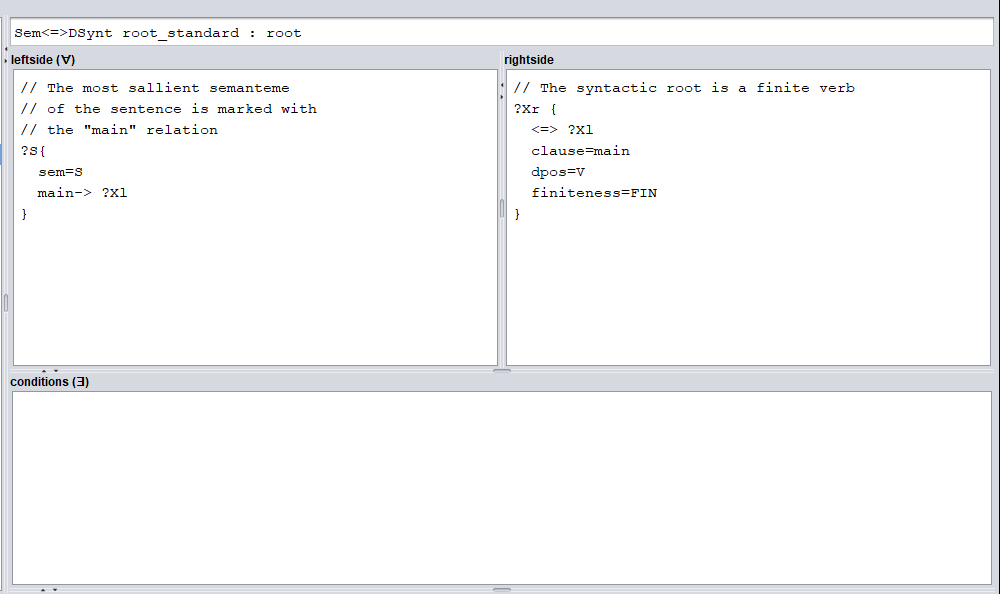
\includegraphics[width=1\textwidth, trim = {0cm 0cm 0cm 0cm},clip]{ch3/figs/grammaire.png}
	\caption{Règle créant la racine syntaxique}
	\label{fig:root}
\end{figure}

%%%%%%%%%%%%%%%%%%%%%%%%%%%%%%%%%%%%%%%%%%%%%%%%
% ---------G R A P H E S ------------------
%%%%%%%%%%%%%%%%%%%%%%%%%%%%%%%%%%%%%%%%%%%%%%%%

\subsubsection{Graphes}\label{entree-sortie}
Maitenant que nous avons fait un survol des dictionnaires et des modules de grammaires, il ne nous reste qu'à présenter les graphes. Dans un premier temps nous présenterons brièvement à quoi ressemble la construction d'un graphe en input. Puis nous montrerons à quoi ressemble les graphes en output.

L'input du réalisateur GenDR est un graphe sémantique de type \acf{TST}. Dans celui-ci les prédicats sont liés à leurs arguments par des relations étiquettées avec des chiffres qui indiquent la position de l'argument. La figure \ref{input} montre comment on construit un graphe sémantique dans MATE.

\begin{lstlisting}[language=XML, caption = Input sémantique, label=input]
structure Sem debt {
S {
owe {
tense=PRES
1-> Paul {class=proper_noun}
2-> "\$500K" {class=amount}
3-> bank {number=SG definiteness=DEF}}
main-> owe}}
\end{lstlisting}

Toutefois, MATE offre aussi une version graphique pour encoder et visualiser le graphe sémantique (voir la figure \ref{fig:graphesem}).
\begin{figure}[htb]
	\centering
	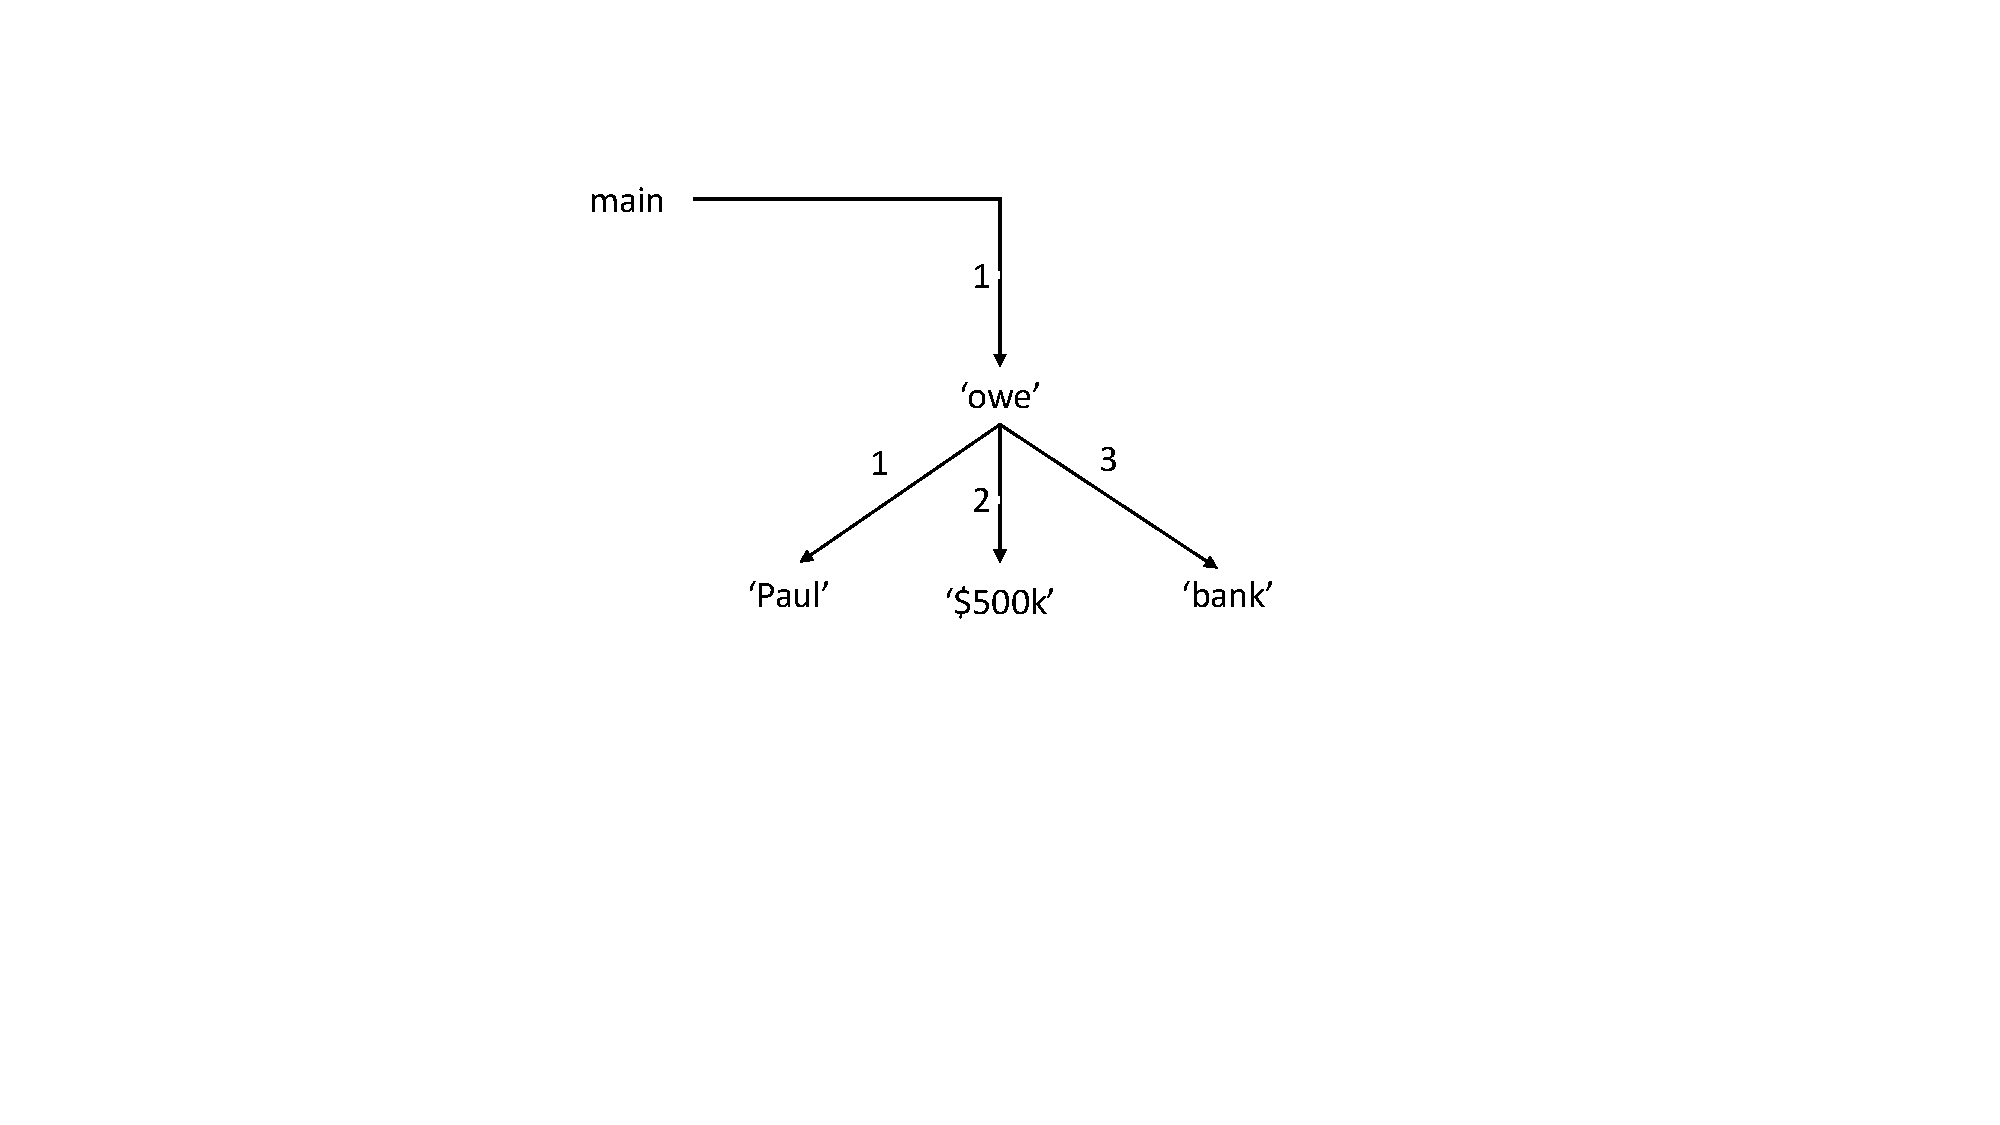
\includegraphics[width=1\textwidth, trim = {0cm 4cm 0cm 3cm},clip]{ch3/figs/owe_sem.pdf}
	\caption{Graphe sémantique en visuel}
	\label{fig:graphesem}
\end{figure}

La section graphe de GenDR nous permet de construire les structures sémantiques d'input et de visualiser les transductions de graphes. Pour l'input donné en \ref{input}, GenDR réalise six structures syntaxiques de surface. Celles-ci peuvent être visualisées dans MATE grâce au module de graphes. La figure \ref{fig:realsurfex} est un exemple d'output visuel que fournirait MATE. 

\begin{figure}[htb]
	\centering
	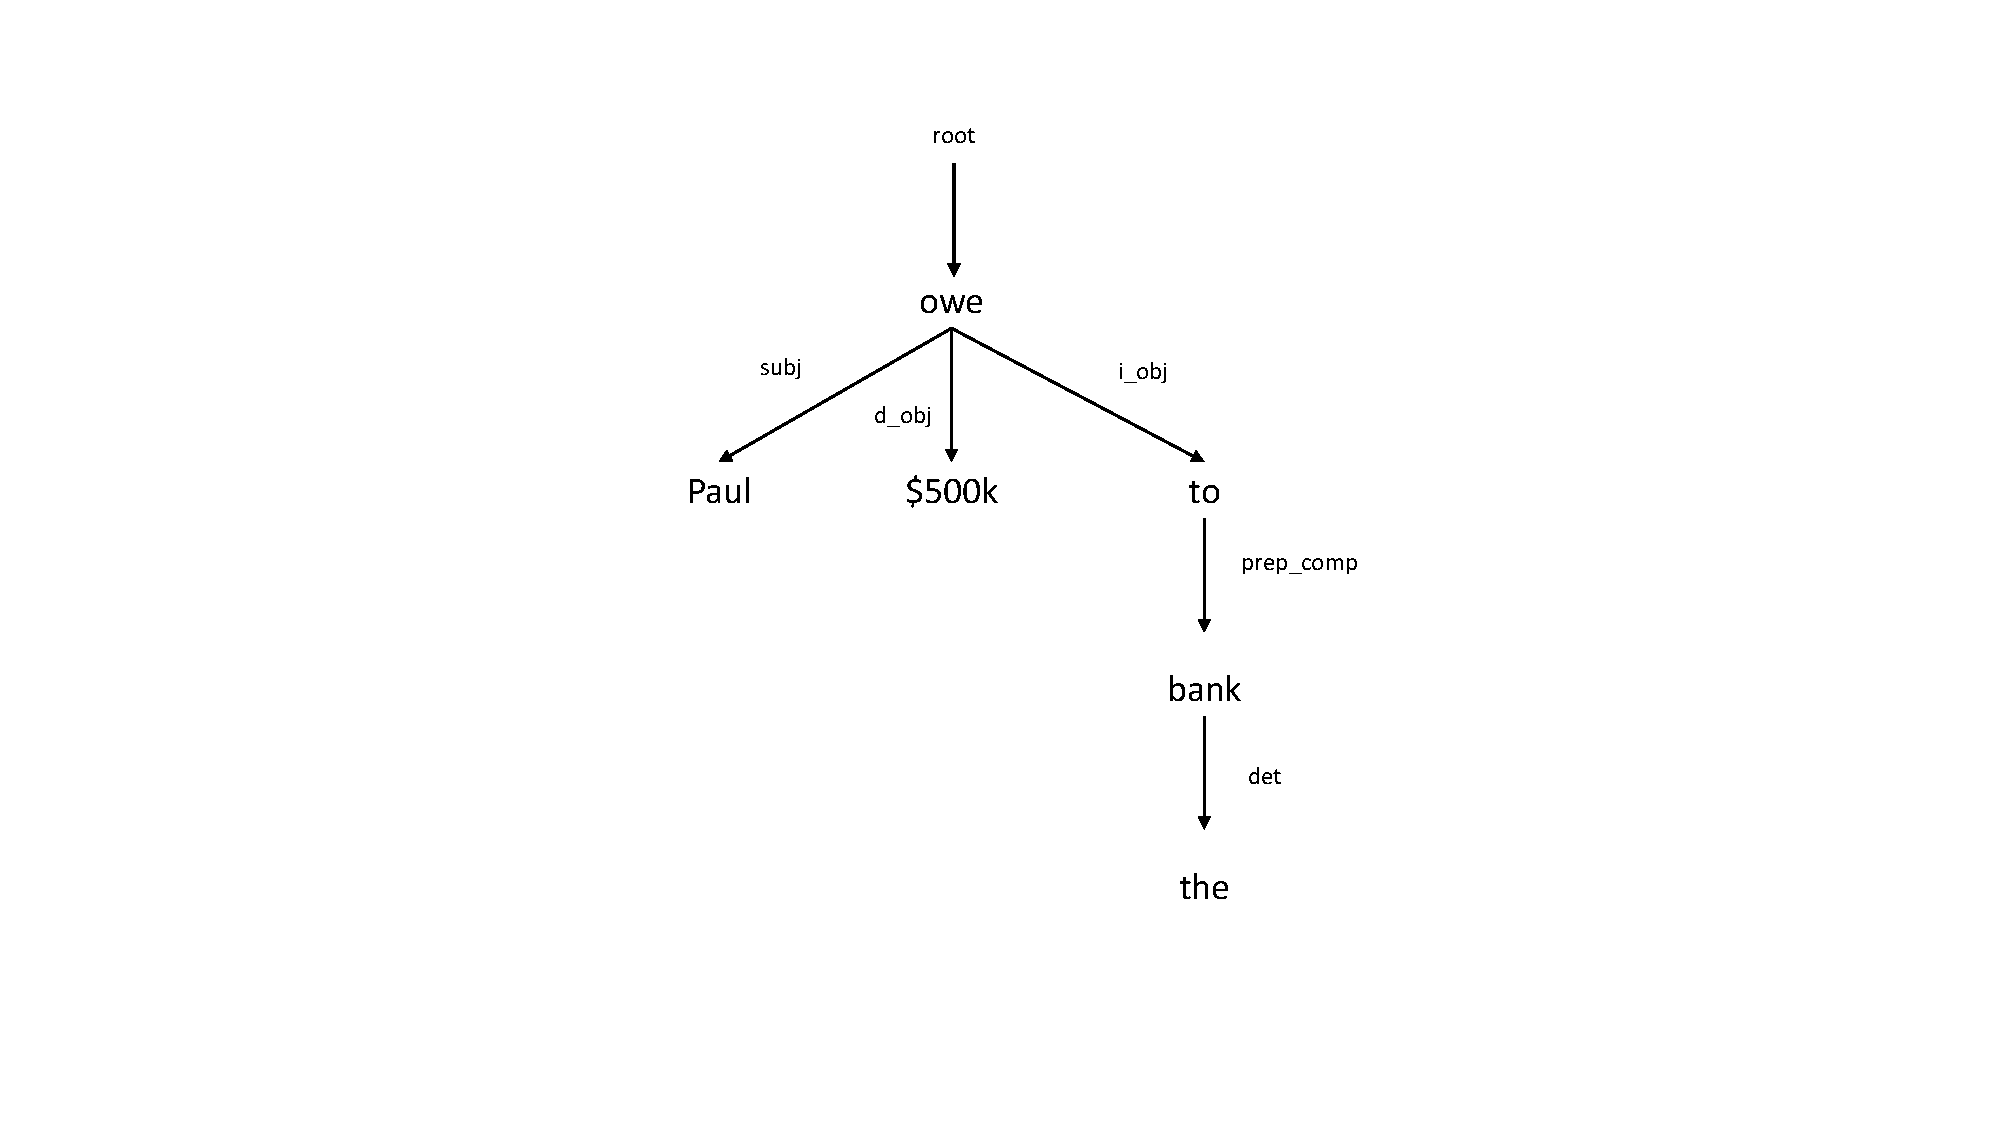
\includegraphics[width=1\textwidth, trim = {0cm 2cm 0cm 2cm},clip]{ch3/figs/realsurfex.pdf}
	\caption{Réalisation de surface}
	\label{fig:realsurfex}
\end{figure}

Toutefois, les modules de règles et de dictionnaires permettent en réalité de réaliser de six arbres syntaxiques superficiels (grâce aux mécanismes de paraphrasage). Nous les présentons à la figure \ref{fig:6realsurf}. Dans cette figure, les arbres de dépendances ont été linéarisés pour faciliter la compréhension du lecteur. Dans les faits, les arbres générés en output ne sont pas linéarisés et ils ressemblent à ceux de la figure \ref{fig:realsurfex}.

\begin{figure}[htb]
	\centering
	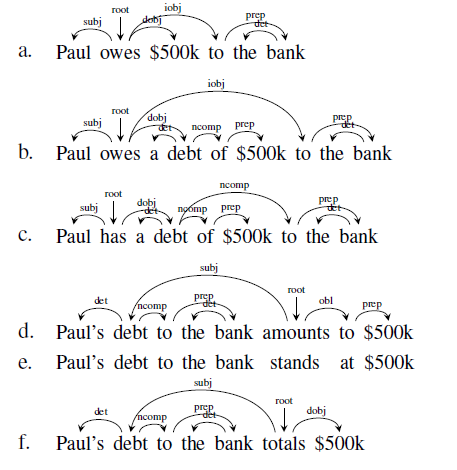
\includegraphics[width=0.5\textwidth, trim = {0cm 0cm 0cm 0cm},clip]{ch3/figs/exemples_real.png}
	\caption{6 réalisations syntaxe de surface}
	\label{fig:6realsurf}
\end{figure}

Si on souhaite une réalisation linéarisée,  il faudra utiliser un réalisateur de surface. GenDR ne traite pas l'interface morpho-syntaxique et ne linéarise pas le texte. C'est exactement dans ces contextes, que les réalisateurs de surface comme SimpleNLG ou JSreal \cite{DaoustJSREALTextRealizer2015}\cite{MolinsJSrealBBilingualText2015}\cite{GattSimpleNLGRealisationEngine2009}entrent en jeu. Au lieu de mettre des efforts à réaliser le texte jusqu'à la fin, GenDR a concentré ses efforts à effectuer des tâches plus abstraites modélisant des phénomènes langagiers complexes. L'arborisation et la lexicalisation sont principalement les deux tâches où GenDR s'est démarqué des autres réalisateurs profonds. Nous les expliquerons en détails dans la section \ref{secsemsynt}.

%%%%%%%%%%%%%%%%%%%%%%%%%%%%%%%%%%%%%%%%%%%%%%%%%%%%%%%%%%%%%%%%%%%%%%%%%%%%%
% --------- I N T E R F A C E   S É M A N T I Q U E- S Y N T A X E ---------
%%%%%%%%%%%%%%%%%%%%%%%%%%%%%%%%%%%%%%%%%%%%%%%%%%%%%%%%%%%%%%%%%%%%%%%%%%%%%

\section{Interface sémantique-syntaxe en TST}\label{secsemsynt}

La capacité de GenDR à réaliser plusieurs phénomèns langagiers découle du travail qui a été fait pour développer son interface sémantique-syntaxe. Dans la section présente, nous décrirons cette interface dans les termes de la \ac{TST}. Plus précisément, nous décrirons deux processus nécessaires au passage de la sémantique à la syntaxe: l'arborisation et la lexicalisation.Pour mieux comprendre ce que sont ces procédés, nous ferons un très bref retour sur la \ac{TST}. 

La \ac{TST} est une théorie qui vise la description de la correspondance entre le \emph{Sens} et le \emph{Texte}. Cette correspondance est effectuée par la construction de modèles formels \citep{PolgueretheorieSensTexte1998}. La figure \ref{fig:modeletst} provient de \citep{PolgueretheorieSensTexte1998} et elle présente comment fonctionnent ces modèles. Elle illustre le fait qu'un modèle Sens-Texte est une machine virtuelle qui prend en entrée des représentations sémantiques d'énoncés et génère un ensemble de Textes qui contiennent toutes les paraphrases permettant d'exprimer le \emph{Sens} donné en entrée. 
\begin{figure}[htb]
	\centering
	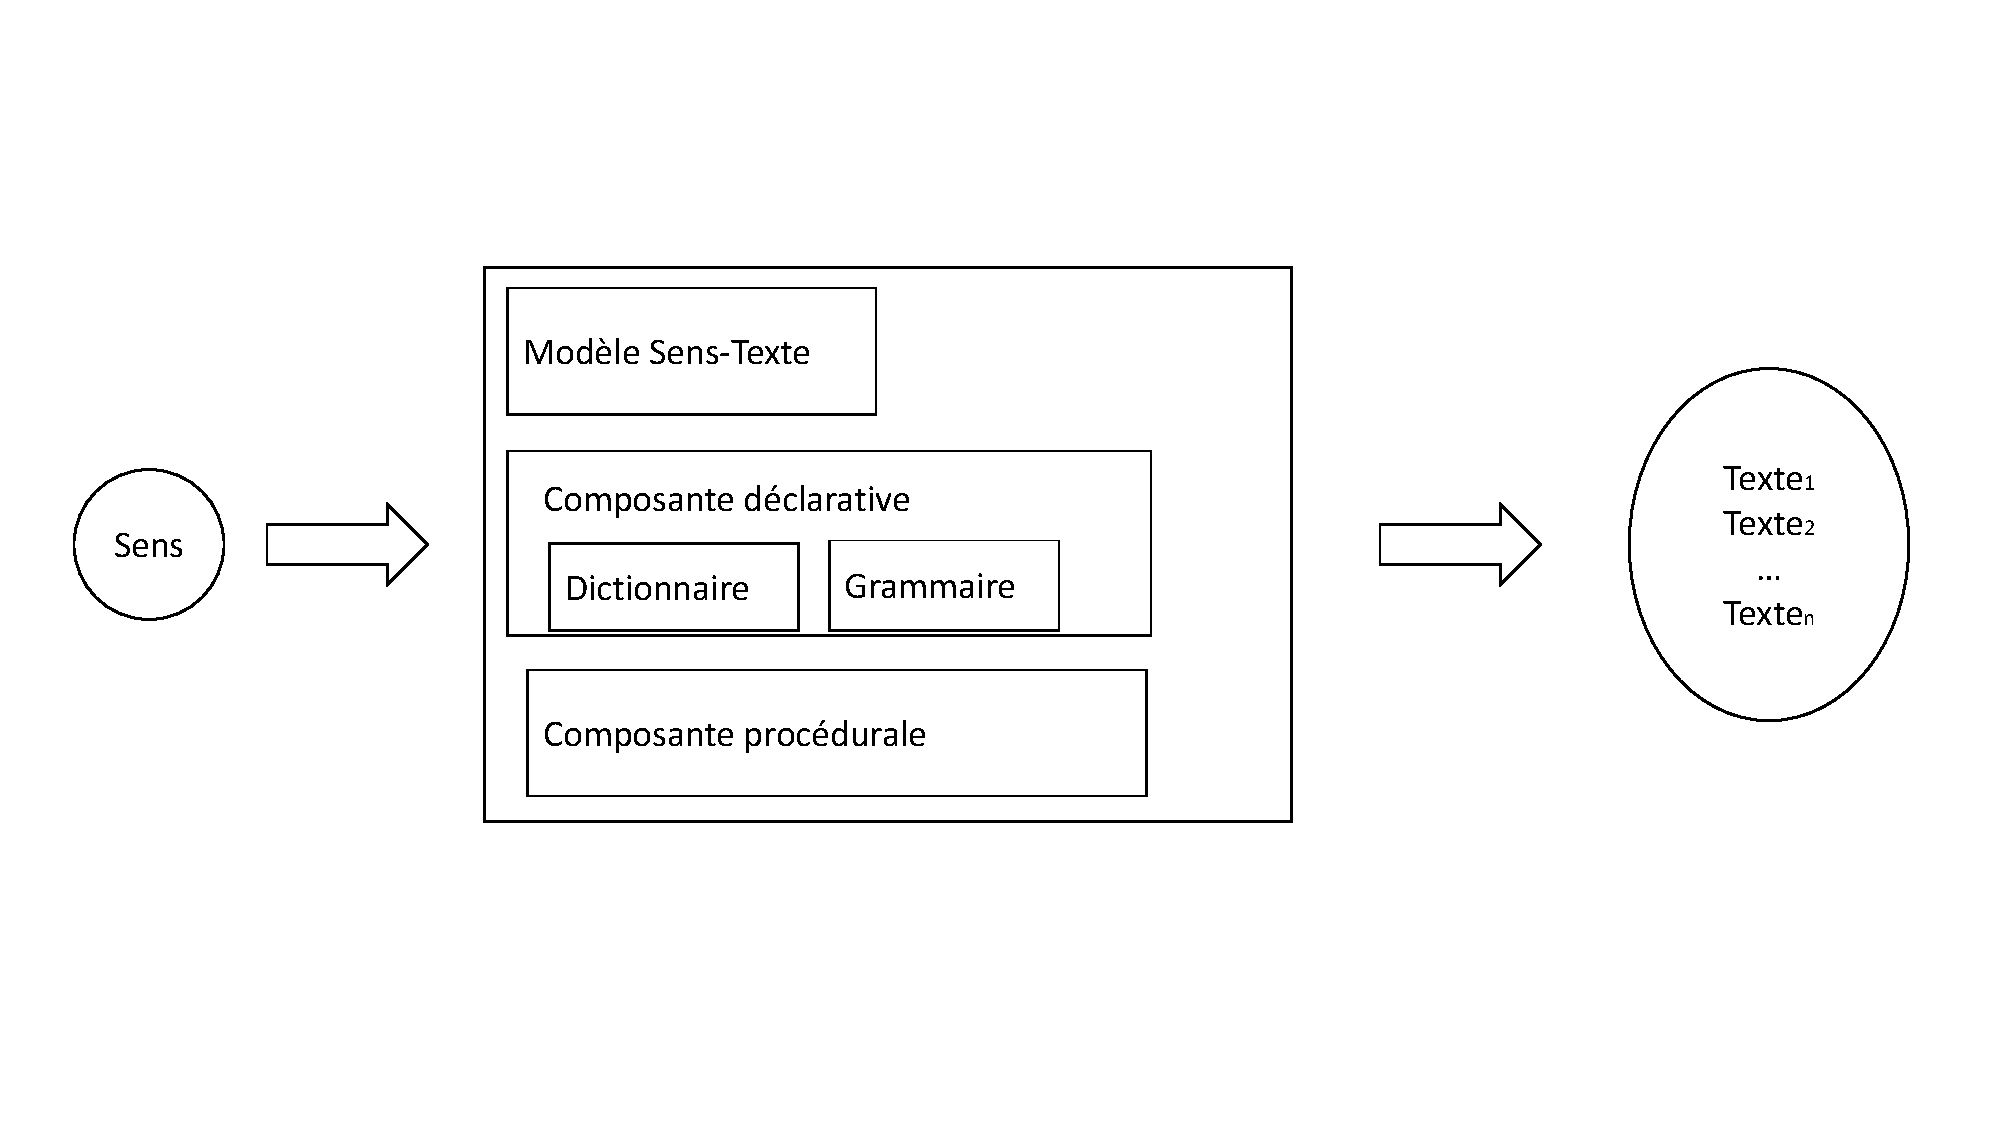
\includegraphics[width=1\textwidth, trim = {0cm 3cm 0cm 3cm},clip]{ch3/figs/polguere1.pdf}
	\caption{Structure d'un modèle TST}
	\label{fig:modeletst}
\end{figure}

Concrètement, la figure \ref{fig:modeletst} démontre comment on passe de la figure 2.4 (qui représente le \emph{Sens}) à la figure 2.6 (qui représente le \emph{Texte}). Pour se rendre au texte final, le \emph{Sens} traverse de nombreux niveaux de représentations. La figure \ref{fig:processustst} démontre les niveaux de représentations que l'input doit traverser succesivement, puis en parallèle comment on représente ces représentations au cours de la réalisation.
\begin{figure}[htb]
	\centering
	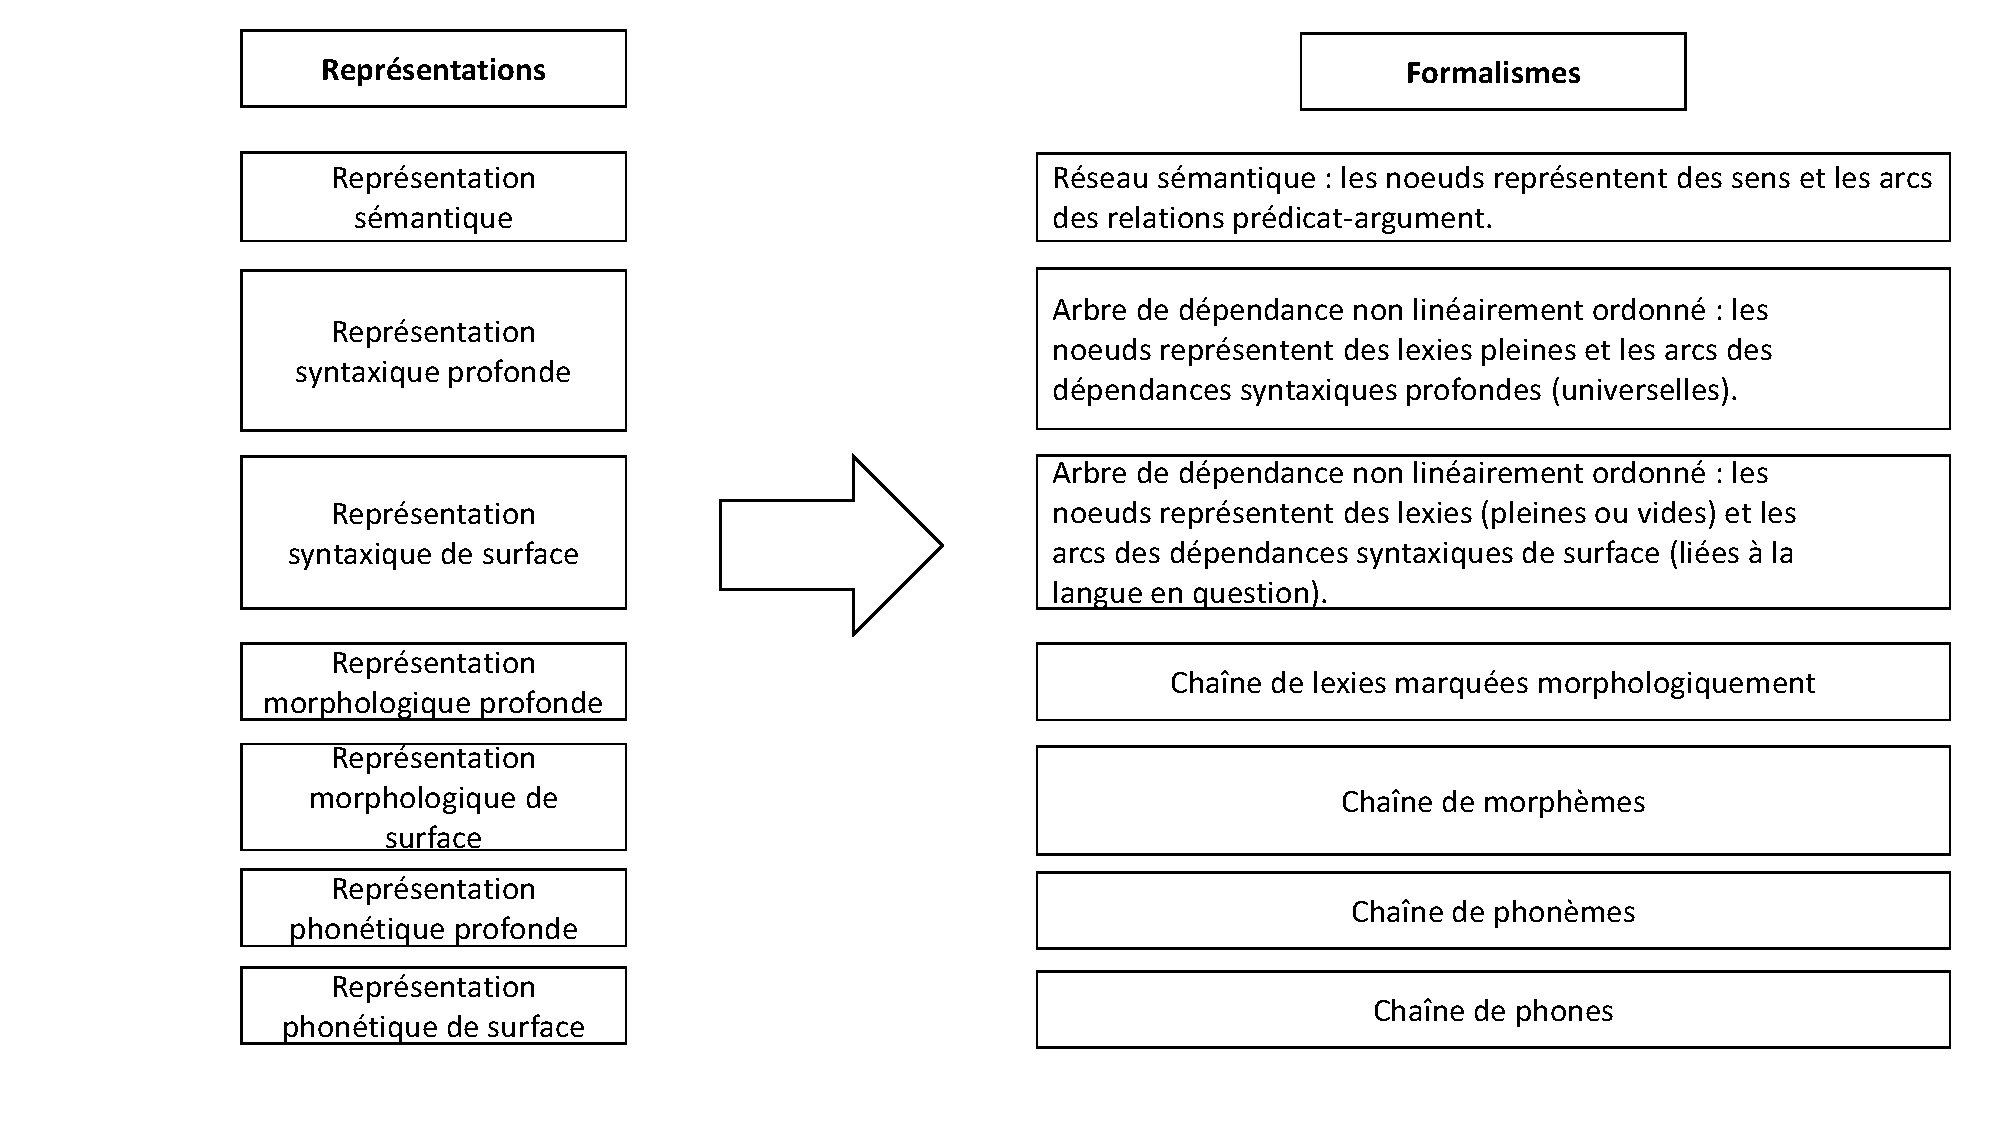
\includegraphics[width=1\textwidth, trim = {0cm 0cm 0cm 0cm},clip]{ch3/figs/polguere2.pdf}
	\caption{Processus d'un modèle TST}
	\label{fig:processustst}
\end{figure}

%%%%%%%%%%%%%%%%%%%%%%%%%%%%%%%%%%%%%%%%%%%%
% ---------T H É O R I Q U E  ------
%%%%%%%%%%%%%%%%%%%%%%%%%%%%%%%%%%%%%%%%%%%

\subsection{Arborisation théorique}\label{arbo}

Comme GenDR traverse trois niveaux de représentations, nous expliquerons uniquement les processus nécessaires à la compréhension du système. Nous commencerons par l'arborisation qui est le passage de la représentation sémantique à la représentation syntaxique profonde.

Selon la \ac{TST}, la structure syntaxique d'un énoncé représente l'ensemble des liens de dependances fonctionnelles qui existent entre les unités lexicales de cet énoncé. On représente formellement ces structures syntaxiques par des arbres qu'on appelle des arbres de dépendances. Cette approche syntaxique provient de \cite{TesniereElementssyntaxestructurale1965} qui est le premier à l'avoir théorisée.

Formellement, le passage de la RSem à la RSyntP se nomme l'arborisation. Elle est ainsi nommée  parce qu'on chercher à arboriser la RSem pour qu'il en résulte un arbre de dépendance profond. Ce passage est effectuée via des règles de correspondance sémantiques. Celles-ci forment une partie de la grammaire dans le schéma montré plutôt à la figure \ref{fig:modeletst}.

Pour que l'arborisation se fasse correctement, il faut que la racine de l'arbre en construction corresponde à un noeud sémantique identifié comme étant le plus saillant. La détermination de la racine correspond au processus de hiérarchisation \citep{PolguereStructurationmisejeu1990}. On l'appelle ainsi car la racine est le noeud qui domine tous les autres noeuds de l'arbre syntaxique profond. Une fois que c'est fait, on va trouver le lexème qui peut satisfaire les contraintes du noeud de la racine. Il faut que le lexème sélectionné corresponde à l'unité sémantique identifiée comme la plus saillante. Le lexème doit aussi satisfaire des contraintes comme la partie du discours ou la finitude. Généralement on a ces contraintes sur la racine puisque ce sont généralement les verbes qui contrôlent les énoncés. En lexicalisant le noeud, on va simultanément ajouté les arcs qui en dépendent. Ceux-ci correspondent aux arguments liés à ce prédicat dans la RSem. Comme \cite{PolguereStructurationmisejeu1990} le dit:
\begin{quotation} chaque arc est considéré successivement dans l'ordre du parcours, puis est traduit en une micro-structure syntaxique profonde grâce aux règles de correspondance sémantique de la grammaire. (p.273)
\end{quotation}

Une fois que l'arborisation est complétée, l'arbre de dépendance profond transitera vers le niveau de syntaxe de surface. Cette transition implique les opérations suivantes. D'abord, faire le calcul des relations syntaxiques de surface. Ainsi, la relation I deviendra sujet, la relation II deviendra complément d'objet direct, etc. De plus, on incorpore les lexies vides (prépositions, déterminants, etc.) à ce stade et on opère la pronominalisation. 

\subsection{Lexicalisation théorique}
Tel que nous l'avions présenté dans la figure \draft{figure dans MARQUIS}, la lexicalisation se produit entre la RSem et la RSyntP \citep{PolguereStructurationmisejeu1990}. Concrètement, il s'agit de la correspondance entre une unité sémantique et les lexies qu'elle contrôle. La correspondance est inscrite dans le dictionnaire sémantique et lexical. La lexicalisation est ainsi très liée à l'arborisation car ce sont deux étapes qui se produisent lors du passage de la RSem à la RSyntP. D'ailleurs, ces deux étapes se produisent successivement l'une à la suite de l'autre. La construction de la représentation syntaxique profonde est une conséquence de l'arborisation des arcs de la RSem et de la lexicalisation des unités sémantiques de cette RSem. Le tout résulte en un arbre de dépendance lexicalisé. Comme nous l'avions vu dans la figure \draft{au début}, le passage de \sem{owe} à \lex{owe} et \lex{debt} représente la lexicalisation.

%%%%%%%%%%%%%%%%%%%%%%%%%%%%%%%%%%%%%%%%%%%%%%%%%%%%%
% --------- C O M P U T A T I O N N E L L E  ------
%%%%%%%%%%%%%%%%%%%%%%%%%%%%%%%%%%%%%%%%%%%%%%%%%%%%

\section{Arborisation et lexicalisation computationnelle}\label{secarbolex}

Maintenant que nous avons présenté le côté théorique de l'interface sémantique-syntaxe, nous exposerons comment ces mécanismes se traduisent d'un point de vue computationnel dans GenDR.

\subsection{Arborisation computationnelle}
La première étape du processus d'arborisation dans GenDR est la même que celle que nous avions expliquée d'un point de vue théorique. Il faut créer la racine de l'arbre qui correspond au noeud le plus saillant de la RSem. Pour faire cela, nous devons indiquer le noeud le plus saillant dans la structure d'input (voir figure x). L'arbre syntaxique profond est construit avec un algorithme top-down qui ressemble beaucoup à celui qu'utilisent MARQUIS et FORGe puisqu'ils sont aussi des tenants de la TST. 

\subsubsection{Règles de base pour l'arborisation}
L'arborisation dans GenDR se fait en trois étapes.

\textbf{Création de la racine}
La première règle appliquée est: root\_standard. Elle construit la racine de l'arbre syntaxique à partir du noeud principal de la structure sémantique. À cette étape, la racine n'est pas étiquettée par un lexème encore (noeud vide), mais on lui impose des contraintes. La contrainte principale est qu'il doit s'agir d'un verbe à l'indicatif. Cette règle ne s'applique donc qu'une seule fois par réalisation.

\textbf{Lexicalisation de la racine}
Une fois que la racine a été créée et contrainte en syntaxe profonde, on applique une règle de lexicalisation. Cela permet au système de fouiller dans les dictionnaires pour un lexème qui correspondra au sens demandé et aux contraintes imposées.

\textbf{Application des règles actancielles}
Une fois que le noeud racine est lexicalisé, GenDR regarde dans le patron de régime de la racine pour savoir comment faire le passage des arcs sémantiques aux arcs syntaxiques. Ceux qui partent du noeud sémantique vers ses arguments seront réalisés comme des actants syntaxiques. Tandis que les arcs qui pointent vers le noeud seront réalisés comme des modificateurs. Bref, les règles qui sont utilisées à cette étape créent de nouveaux noeuds et de nouveaux arcs en partance de la racine. Ces noeuds se font imposer des contraintes par le patron de régime du gouverneur (la racine) et les lexies qui satisferont ces contraintes pourront être lexicalisés. C'est ainsi qu'on retourne à la seconde étape pour lexicaliser ces noeuds. Puis cycliquement, nous retournons à la troisième étape puisque de nouveaux noeuds lexicalisés amènent leur patron de régime avec eux. Et ce jusqu'à ce que le graphe sémantique soit complètement réalisé en surface profonde. Les règles sémantiques qui s'occupent de cela sont: actant\_gp, actant\_guess, attr\_lex. 

\subsection{Lexicalisation computationnelle}
La lexicalisation dans GenDR implique trois niveaux de représentations (RSem, RSyntP et RSyntS) et se fait en deux étapes. La lexicalisation profonde est la première des deux étapes. Il s'agit de faire correspondre une unité sémantique à une unité lexicale profonde. Cette phase introduit des lexies pleines de sens. S'ensuit la lexicalisation de surface qui consiste à introduire les mots fonctionnels et les lexies de surface. La phase de lexicalisation s'opère grâce à des ressources lexicales: des dictionnaires et des règles de lexicalisation. Ainsi, la sélection de l'unité lexicale profonde pour réaliser l'unité sémantique fournie en input se fait en consultant les dictionnaires lexicaux. Dans GenDR, nous deux dictionnaires servant contribuant à l'étape de lexicalisation. Nous avons d'abord, le dictionnaire sémantique, puis le dictionnaire lexémique et un dictionnaire de fonction lexicale. Il s'agit de ceux qui ont été présentés en \ref{dictio}. En ce qui concerne les règles. Nous décrirons, dans cette section, quelques règles de lexicalisation de base. Nous omettrons les règles de lexicalisation complexes (collocations, expressions idiomatiques, etc.) car ce n'est pas le propos de ce mémoire. Pour plus d'informations concernant celles-ci nous vous référons à Lambrey et Lambrey, Lareau et Lareau,al.

\textbf{Les lexicalisations simples}
sont traitées par la règle \emph{lexicalization\_standard}. Cette règle prend une unité sémantique donnée dans un graphe sémantique et vérifie dans le dictionnaire sémantique quelles sont les correspondances lexicales de ce sémantème (tel que démontré en \ref{semanticon}). Puis le système récupère toutes les lexicalisations possibles de l'unité sémantique. S'ensuit la sélection de l'unité lexicale. Pour ce faire, GenDR s'assure que la partie du discours profonde de la (ou les) lexie(s) correspond à celle qui est demandée sur le noeud contraint dans l'arbre syntaxique profond en construction. Effectivement, si la lexie satisfait les contraintes du noeud, alors GenDR permet la lexicalisation. L'arbre syntaxique profond sera désormais doté d'un noeud consommé par cette lexie choisie. D'ailleurs, c'est ce mécanisme qui permet le paraphrasage. Puisque le système créera autant d'arbres syntaxiques profonds qu'il y a de lexies possibles pour un noeud donné. 

\textbf{Lexicalisation de classes}
Les classes comme les chiffres, les montants, les noms propres ou les acronymes ont une règle de lexicalisation particulière. Il s'agit d'une règle qui se charge des unités sémantiques que nous ne voulons pas nos dictionnaires sémantiques et lexicaux. D'abord, parce qu'elles sont trop nombreuses et parce que leur comportement est prévisible. Pour déclencher l'application de cette règle, on précise dans la structure d'input à quelle classe le sémantème appartient. Les traits lexicaux (DPOS, etc.) de ces classes sont encodés dans le lexicon.

\textbf{Lexicalisation de secours}\label{secours}
Les règles de lexicalisation de secours permettent à GenDR de lexicaliser une unité sémantique ou lexicale dont il n'a pas les informations. Puisque le système possède les 1500 lexies les plus fréquentes de l'anglais, il est évident que certaines lexies ou sémantèmes manqueront à l'appel. Pour remédier à la situation, il y a deux mécanismes. D'abord, si le sémantème dans l'input a existe sous la même forme dans le lexicon, alors le système va lexicaliser le sémantème avec ce lexème. Cela a comme conséquence qu'on n'a pas besoin d'inscrire le sémantème dans le semanticon s'il n'y a qu'une lexicalisation possible de celui-ci (cela permet de sauver du temps). Cependant, si le sémantème ne figure pas dans le lexicon, alors le système fait une supposition \draft{ma traduction de 'take a guess', mais j'pas certain que c'est bon}. Il va supposer que l'étiquette de l'unité sémantique est la même que l'unité lexicale et s'il y a des contraintes sur le noeud d'arrivée, alors le système suppose que l'unité qu'il suppose satisfait les contraintes. Les lexèmes devinés seront mis en évidence dans la réalisation d'output afin que l'utilisateur sache qu'une règle de lexicalisation de secours a été employée.
	
\textbf{Lexicalisation grammaticale}
Les règles de lexicalisation précédentes prenaient place entre la Rsem et la RSyntP. Les règles de lexicalisation grammaticale prennent au place au niveau syntaxique superficiel (RSyntS). Elles introduisent des lexèmes fonctionnels. Il y a des règles qui introduisent les lexèmes exprimant des sens grammaticaux comme les auxiliaires et les déterminants. Ces règles sont déclenchées par la précision des sens grammaticaux dans les structures d'input (voir la figure exemple). Ces lexèmes existent en syntaxe profonde, mais on ne les voit pas sous forme de noeuds, mais plutôt sous forme de traits. Comme ces mots appartiennent à une classe fermée et qu'ils sont peu nombreux et souvent spécifiques à une langue, ce sont donc des règles particulières qui traitent ces lexiclaisaiton dans chaque module de langue. Puis, il y a des règles de lexicalisation grammaticales s'occupant des lexèmes sélectionnés par les patrons de régime (comme les prépositions). Ces lexèmes sélectionnés sont introduits en syntaxe comme des noeuds extra entre un gouverneur et son dépendant. Ils sont donc encodés dans le patron de régime du gouverneur.

%%%%%%%%%%%%%%%%%%%%%%%%%%%%%%%%%%%%%
% --------- E X E M P L E ---------
%%%%%%%%%%%%%%%%%%%%%%%%%%%%%%%%%%%%%

\section{Exemple}\label{secexemple}

Pour illustrer le fonctionnement des règles et des dictionnaires que nous avons présenté, nous décortiquerons la réalisation profonde de l'exemple vu à la figure~\ref{input}.

\subsection{1ère phase: RSem à RSyntP}
Cette section illustre les étapes successives qui ont permis à GenDR de passer de la \ac{RSem} à la \ac{RSyntP}. Il s'agit de l'arborisation profonde et de la lexicalisation profonde.

\subsubsection{Application de la règle \emph{root\_standard}}
La règle crée un noeud vide qui sera la racine de l'arbre à construire. Ce noeud est contraint par deux traits et il demande un verbe fini. La figure \ref{fig:rootstand} illustre la création du noeud non-étiquetté.
\begin{figure}[htb]
	\centering
	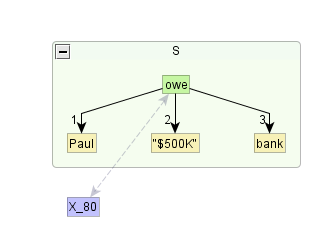
\includegraphics[width=0.6\textwidth, trim = {0cm 0cm 0cm 0cm},clip]{ch3/figs/inspecteur_root.png}
	\vspace{-0.5cm}
	\caption{Application de root\_standard}
	\label{fig:rootstand}
\end{figure}

\subsubsection{Application de la règle \emph{lex\_standard}}
Ensuite, on procède à la lexicalisation de la racine. Le sémantème \sem{owe} renferme deux lexèmes possibles \lex{owe} et \lex{debt}. GenDR va donc tenter de combler la racine avec ces deux lexèmes. Les deux sont possibles. Le système peut lexicaliser la racine en choisissant \lex{debt} car ce nom commun encode une fonction lexicale lui permettant de s'unir à un verbe support pour représenter le sens \sem{owe}. Mais il s'agit d'une lexicalisation complexe et nous vous renvoyons à Lambrey, Lareau pour cela. Le système peut donc aussi lexicaliser la racine en choisissant le verbe \lex{owe}.

\begin{figure}[htb]
	\centering
	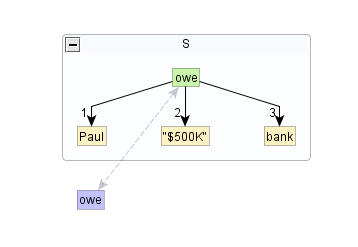
\includegraphics[width=0.7\textwidth, trim = {0cm 0cm 0cm 0cm},clip]{ch3/figs/lex_standard_root.png}
		\vspace{-0.5cm}
	\caption{Application de lex\_standard}
	\label{fig:lexstand1}
\end{figure}

\subsubsection{Application de la règle \emph{actant\_gp}}
Une fois que la racine est pourvue d'un lexème, l'application de la règle actant\_gp est déclenchée. Pour chaque relation actancielle, le système puise dans le patron de régime de \lex{owe} et il effectue la conversion des actants sémantiques en actants syntaxiques. Dans l'input (figure \ref{input}), \sem{owe} possède trois actants sémantiques. Ils seront réalisés en actants syntaxiques en fonction de la diathèse imposée par l'entrée \lex{owe}. Brièvement, la diathèse est la correspondance entre les actants sémantiques et syntaxiques. Puis les noeuds au bout des arcs syntaxiques seront contraints en fonction des restrictions prévues par le patron de régime de \lex{owe} pour chacun de ses actants syntaxiques. Le patron de régime du verbe demande que deux de ses actants syntaxiques sont de type dpos=N et un de type dpos=Num. Cela nous permet de nous assurer que les noeuds qui seront lexicalisés sont permis par le dictionnaire. Nous élaborerons plus en détails sur les notions de patron de régime et diathèse à la section \ref{sectiongp}. \lstinline!(gp = {1=I 2=II 3=III} et (I={dpos=N} and III={dpos=N})!, et l'actant II est soit un montant ou un nombre (II={dpos=Num}).
\begin{figure}[htb]
	\centering
	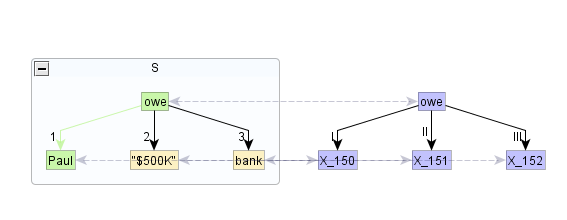
\includegraphics[width=1\textwidth, trim = {0cm 0cm 0cm 0cm},clip]{ch3/figs/actant_gp1.png}
	\caption{Application de actant\_gp}
	\label{fig:actantgp}
\end{figure}

\subsubsection{lex class et lex standard}
Puisque nous sommes rendu avec de nouveaux noeuds non-étiquettés, il faut répéter la phase de lexicalisation. On devra donc trouver les lexèmes correpondants aux entrées \sem{Paul}, \sem{bank} et \sem{\$500}. À cette étape, GenDR utilise deux règles de lexicalisation différentes: une règle de lexicalisation pour les classes(\emph{lex\_class}) et une règle de lexicalisation standard(\emph{lex\_standard}). Il utilise \emph{lex\_class} car \sem{Paul} et \sem{\$500} ont des traits \emph{class} dans l'input sémantique.Elle passer directement au lexicon, puisque les sens ne sont pas encodés dans le semanticon comme les classes ont des comportements prédictibles. Dans le lexicon par contre, c'est là que les classes sont décrites. Effectivement la classe proper\_noun et la classe numeral vont permettre l'application de la règle lex\_class et de lexicaliser paul et 500 piastres. Les classes ont les informations de type dpos et autres traits grammaticaux. L'étiquette du noeud sémantique est directement copiée en syntaxe. on s'assure finalement que les contraintes de ces classes respectent les contraintes du noeuds généré par gp\_actant. Lorsque c'est le cas, la lexicalisation se produit. Les noms propres héritent des traits de la classe des noms, donc la dpos est là, puis les montants héritent des traits de la classe des nombres. Ensuite le système utilise \emph{lex\_standard} pour lexicaliser \sem{bank}. Le processus est le même que nous avons décrit pour la première occurrence de cette règle.\lex{bank} sera lexicalisé comme III actant syntaxique puisqu'il correspond au sens \sem{bank} et parce qu'il satisfait les contraintes du noeud imposées par la règle \emph{actant\_gp}.

\begin{figure}[htb]
	\centering
	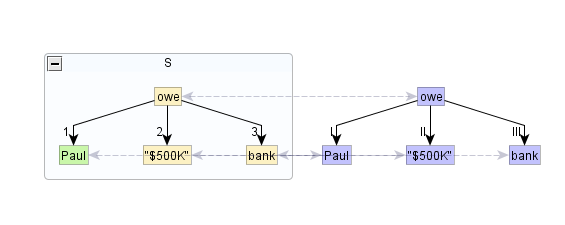
\includegraphics[width=1\textwidth, trim = {0cm 0cm 0cm 0cm},clip]{ch3/figs/lex_standard2.png}
	\caption{Application de lex\_standard}
	\label{fig:lexstand2}
\end{figure}

\subsection{2ème phase: RSyntP à RSyntS}

\subsubsection{Application des règles de lexicalisation de surface}
On va chercher les lexicalisations de surface de chacune des unités lexicales avec les règles \emph{lex\_class} et \emph{lex\_lu}. La première se charge de lexicaliser en surface les unités de type classe et la seconde les unités normales.
\begin{figure}[htb]
	\centering
	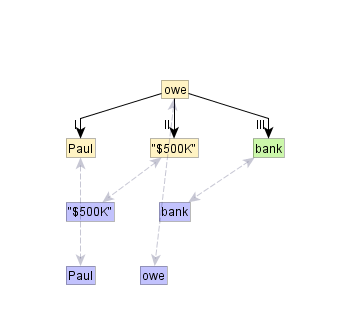
\includegraphics[width=0.7\textwidth, trim = {0cm 0cm 0cm 0cm},clip]{ch3/figs/rsyntslexicalisation1.png}
	\caption{Application de lex class et lex lu}
	\label{fig:lexsurf}
\end{figure}

\subsubsection{Application des règles actancielles de surface}
Ensuite, les règles actancielles de surface s'appliquent. Concrètement, ces règles remplacent les étiquettes des arcs de l'arborisation profonde (I, II, III,...) par des étiquettes de syntaxe de surface (sujet, objet direct, objet indirect,...). Ces étiquettes de surface sont encodées dans le patron de régime du verbe qui gouverne les actants syntaxiques. Ainsi, la relation subjectale est réalisée par la règle \emph{actant\_subj}. Qui réalise la relation entre le sujet et le verbe. Cette information est encodée dans le gp du verbe \lex{owe} qui hérite des traits de la classe verb\_dit. Celle-ci hérite des traits de la classe verb\_dt qui hérite des traits de la classe verb. C'est dans celle-ci que se trouve l'information nécessaire à l'application de la règle \lstinline!gp = { I = { dpos = N rel = subjective } } !. Ainsi, on voit encore comment le dictionnaire et les règles sont inter-reliés. Pour que la règle actant\_subj s'applique au sujet de la structure, elle va regarder dans la dictionnaire à quel actant syntaxique elle doit faire le lien. Elle ne prend que l'actant syntaxique qui précise la relation subjective.

Les mêmes phénomènes s'appliquent ensuite pour les règles \emph{actant\_dir} et \emph{actant\_prep}. Toutefois, la règle \emph{actant\_prep} diffère des deux autres règles actancielles car elle crée un noeud intermédiaire en syntaxe de surface pour accueillir le lexème fonctionnel \lex{to} qui est nécessaire à la bonne formation de la phrase. La nature de la préposition est encodée dans le gp du verbe ainsi \lstinline! gp = {III = { dpos = N  rel = indir_objective  prep = to }  }!.

\subsubsection{Application de la règle des déterminants}

La règle \emph{det\_def} ajoute les déterminants aux lexèmes en fonction de leur définitude. Parmi les règles que nous avons présenté, c'est la seule règle de GenDR qui est propre à l'anglais. Elle lexicalise \lex{the} puisque l'unité sémantique \sem{bank} était marquée par le trait défini dans la structure d'input.

La figure \ref{fig:syntsurf} démontre l'application simultanée des règles actancielles et de la règle des déterminants.

\begin{figure}[htb]
	\centering
	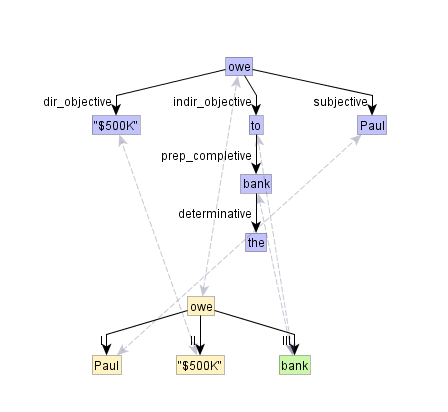
\includegraphics[width=0.7\textwidth, trim = {0cm 0cm 0cm 0cm},clip]{ch3/figs/rsynts_syntactisation.png}
	\caption{Application de subj,dir,prep et det}
	\label{fig:syntsurf}
\end{figure}

%%%%%%%%%%%%%%%%%%%%%%%%%%%%%%%%%%%%%%%%%%%%%%%%
% --------- P R O B L É M A T I Q U E ---------
%%%%%%%%%%%%%%%%%%%%%%%%%%%%%%%%%%%%%%%%%%%%%%%%

\section{Problématique}\label{problema}

La démonstration précédente prouve que GenDR performe très bien en ce qui concerne les phénomènes langagiers complexes et profonds. Toutefois, le dictionnaire lexical de ce système ne couvre que les 1500 lexies les plus fréquentes du langage. Pour offrir une couverture encore plus importante du langage, il faudrait que GenDR acquière beaucoup plus d'entrées lexicales. Plus particulièrement les verbes car ce sont eux qui contrôlent la structure d'une phrase (ce qui est confirmé par la règle d'arborisation de création de la racine propre à MARQUIS, FORGe et GenDR). Comme \cite{SchulerVerbnetBroadcoverageComprehensive2005} le dit dans sa thèse:

\begin{quotation} In particular, since verbs often convey the main idea of a sentence, such a resource must represent verb meanings. These require a particularly precise and well deffined representation that captures both their predicate-argument structure as well as their semantic content\end{quotation}.

Nous sommes en accord avec cette déclaration et nous pensons qu'une ressource comme GenDR bénéficierait grandement d'une large couverture des verbes dans le cadre de la réalisation profonde. Parmi les 1500 lexies de l'anglais, 500 sont des verbes. Cela est non-négligeable mais, il est clair que GenDR gagnerait en couverture linguistique s'il se dotait d'une ressource lexicale lui permettant de traiter plus de verbes.

La raison d'être de ce mémoire prend place dans ce contexte. Tout comme \cite{SchulerVerbnetBroadcoverageComprehensive2005}, \cite{Korhonenlargesubcategorizationlexicon2006} et \cite{MESSIANT08.142} suggèrent aussi que la représentation des langues naturelles en \ac{TAL} passe par des ressources lexicales décrivant les comportements syntaxiques des lexèmes. Grâce à un dictionnaire verbal, GenDR pourrait couvrir une grande partie de langue anglaise. C'est pourquoi nous avons tenté d'implémenter un dictionnaire décrivant les comportements syntaxiques des verbes (aussi appelés patrons de régime, cadre valenciel, cadre de sous-catégorisation,etc.).

\section{Patrons de régime}\label{sectiongp}

\draft{refaire tout ce paragraphe:
Pour mieux comprendre l'utilité d'un tel dictionnaire, il faut expliquer ce sont les patrons de régime. Dans l'exemple plus haut, nous avons vu comment les patrons de régime permettaient l'arborisation. Les patrons de régime décrivent les cooccurrences syntaxiques des unités lexicales \citep{MilicevicSchemaregimepont2009}. La cooccurrence de la lexie avec ses actants. Autrement dit les sujets et objets des verbes, les compléments du nom. Ceux-ci correspondent aux actants syntaxiques de surface. Le patron de régime encode des relations plus profondes comme les actants syntaxiques profonds. Les patrons de régime d'une lexie correspondent à l'ensemble des constructions syntaxiques dont la lexie est la gouverneure. Les actants syntaxiques en sont ses dépendants. On les encode dans un dictionnaire car les patrons de régime des lexies ne sont généralement pas prévisibles. Effectivement, on ne peut pas prédire les patrons de régime des unités lexicales d'une langue. D'ailleurs, même des verbes sémantiquement proches ne possèderont pas nécessairement les mêmes constructions syntaxiques ex de Milicevic p. 95( se souvenir de X , mais se rappeler X ). Le nombre d'actant n'est pas prévisible non plus en regardant l'unité lexicale à partir de son sens. 

Puisque les arguments sélectionnés par une lexie sont généralement idiosyncratiques, on encode ces comportements syntaxiques dans des dictionnaires.

les GP encodent la diathèse (correspondance entre les actants sémantiques d'une lexie et ses actants syntaxiques profonds) et la réalisation des actants (I à sujet II objet direct, indirect, ou oblique). La diathèse peut soit être triviale (1 pour I, 2 pour II, etc.) ou pas (1 -II et 2-I)

Le patron de régime d'une lexie encode les correspondances entre ses actants (au niveau sémantique, syntaxique profond et syntaxique de surface), les moyens morpho-syntaxiques d'expressions des actants et les restriction sur les actants.

Plus tôt dans le chapitre nous avions parlé de l'interface sémantique-syntaxe et de l'importance des règles sémantiques qui font la transition entre Rsem et RSyntP. Le rôle le plus important du GP est de fournir l'information nécessaire au passage de la sem à la synt lors des opérations de lexicalisation et d’arborisation. 
}
\begin{quotation}{Comme le choix lexical détermine le choix des constructions syntaxiques possibles (la lexie sélectionnée « amène » avec elle son régime) et vice-versa (le choix d’une structure impose certains choix lexicaux), on peut dire que c’est le schéma de régime qui, au sein d’un MST, fait le pont entre le lexique et la grammaire. \citep{MilicevicSchemaregimepont2009}, p.105}
\end{quotation}

\draft{faire une meilleure transition ici}GenDR bénéficierait énormément d'un dictionnaire de patron de régime. Notamment parce que le logiciel MATE présente des limites d'encodage quant à la manière dont les gp sont encodés présentement dans GenDR. Pour un verbe donné, on ne peut pas avoir deux parties du discours différentes qui compétitionnent pour la même position syntaxique. Autrement dit, prenons le cas de X (exemple). Cela restreint le nombre de génération possible pour un verbe ou bien ça peuple inutilement le dictionnaire d'entrée verbale par partie du discours qu'il prend. Ce n'est pas une manière efficace d'encoder le langage. C'est là qu'un dictionnaire de patron de régime entre en ligne de compte. Et ça permet une grande couverture de la langue. Sans dictionnaire de patron de régime ni d'acquisition automatique de ceux-ci, il faut les encoder à la main un par un. Ce n'est pas une tâche rationnelle. C'est ainsi que plusieurs groupes de recherches ont voulu remédier à cette situation. Plusieurs s'entendent pour dire qu'un meilleur traitement du \ac{TAL} se fait grâce à des ressources lexicales riches. C'est pour cette raison que nous avons pensé implémenter un dictionnaire de verbe à GenDR pour le rendre plus performant. Nous nous sommes finalement retourner vers VerbNet, une ressource lexicale très riche.